\chapter{Réalisation}
La phase de réalisation est la phase opérationnelle de la création d’un système informatique.
Elle consiste à la concrétisation et la matérialisation de toutes les phases
d’analyse au niveau graphique et technique.  Dans ce chapitre, nous commençons par
une description de l’environnement matériel, logiciel et de programmation. Nous enchaînons
par une étude comparative afin de justifier le choix des technologies adoptées. Par la suite, 
nous présentons quelques interfaces des modules réalisés, afin d’illustrer leurs fonctionnalités
principales.

\section{Environnement de travail}

Nous décrivons dans cette section l’environnement matériel et logiciel adopté pour l’implémentation de notre application.

\subsection{Environnement matériel}

{\bf Station de travail 1 :}\\
Marque: PC portable HP\\
Processeur: Intel Core i7 CPU\\
Mémoire: 8,00GO de RAM\\
Type système d'exploitation : Windows 10.\\
~\\

{\bf Station de travail 2 :}\\
Marque: Serveur HP ProLiant DL380 G7 \\ 
Processeur: 2 x Intel Xeon E5450\\
Mémoire: 4,00Go de RAM\\
Type système d'exploitation : Windows Server 2008 R2.\\

\subsection{Environnement logiciel}
Tout le long de la phase de développement, nous nous sommes servies de l’environnement
logiciel suivant :\\
\begin{description}

{\bf \item Cloud9 IDE :} 
Cloud9 IDE est un environnement de développement intégré en ligne, publié en open source de la version 3.0. Il prend en charge des centaines de langages de programmation, y compris C, C ++, PHP, Ruby, Perl, Python, JavaScript avec Node.js et Go. Il permet aux développeurs pour commencer avec le codage immédiatement avec des espaces de travail pré-configurés, collaborer avec leurs pairs avec des fonctionnalités de codage de collaboration, et les caractéristiques de développement web comme la prévisualisation en direct et les tests de compatibilité du navigateur. [Langage promotionnel]
Il est écrit presque entièrement en JavaScript, et utilise Node.js sur le back-end. Le composant éditeur utilise Ace. En Juillet 2014, il utilise des conteneurs de Docker pour ses espaces de travail, et est hébergé sur Google Compute Engine.
{\bf \item SQL*Plus : }SQL*Plus est un utilitaire en ligne de commande d'Oracle qui permet aux utilisateurs d'exécuter interactivement des commandes SQL et PL/SQL. Décliné en plusieurs versions (graphique et web), il est principalement distribué avec le produit Oracle Database.
{\bf \item SublimeText : }
Sublime Text est un éditeur de texte générique codé en C++ et Python, disponible sur Windows, Mac et Linux. Le logiciel a été conçu tout d'abord comme une extension pour Vim, riche en fonctionnalités.
Depuis la version 2.0, sortie le 26 juin 2012, l'éditeur prend en charge 44 langages de programmation majeurs, tandis que des plugins sont souvent disponibles pour les langages plus rares.
{\bf \item StarUML : }
c'est un logiciel open-source cédé par son ancien éditeur sous licence GNU GPL, dédié aux plate-formes Windows, il est développé en Delphi. Ses principaux avantages
sont sa simplicité d’installation et de prise en main, et la possibilité de générer le squelette
des classes en langages Java, C++, ActionScript3.0. De plus, le logiciel a été conçu en prévoyant l’ajout de plugin supplémentaire afin de pouvoir être adapté simplement aux besoins évolutifs de ses utilisateurs. Enfin StarUML gère l’exportation des données au format XMI, le standard pour l’échange d’informations de métadonnées UML basé sur XML, ainsi que l’exportation au format jpg afin d’intégrer les diagrammes au sein des  documents.
{\bf \item Texmaker :}
c'est un logiciel libre destiné à l'édition de documents LaTeX et fonctionnant sur GNU/Linux, Mac OS X, Windows et OS/2. Il est développé en C++ à l'aide de la bibliothèque Qt.
Cet éditeur offre un lot de fonctionnalités : support complet de l'Unicode, coloration syntaxique, correction orthographique lors de la frappe, auto complétion, pliage/dépliage de code, snippets, support des expressions régulières, sélection rectangulaire, gestionnaire de session...
\end{description}
\subsection{Les choix techniques }
Nous discutons dans ce paragraphe les choix technologiques adoptés pour le développement.
\begin{description}
{\bf \item Laravel :}
 Laravel est un framework web open-source écrit en PHP respectant le principe modèle-vue-contrôleur et entièrement développé en programmation orientée objet. Laravel est distribué sous licence MIT, avec ses sources hébergées sur GitHub. Laravel, créé par Taylor Otwel, initie une nouvelle façon de concevoir un framework en utilisant ce qui existe de mieux pour chaque fonctionnalité\cite{cite2}.
{\bf \item Microsoft SQL Server :}
Microsoft SQL Server est un système de gestion de base de données (abrégé en SGBD) incorporant entre autres un SGBDR (SGBD relationnel ») développé et commercialisé par la société Microsoft. Il ne fonctionne que sous les OS Windows. En fait MS SQL Server est une suite composée de cinq services principaux :\\
Le moteur relationnel (OLTP) appelé SQL Server ;\\
Le moteur décisionnel (OLAP) appelé SSAS (SQL Server Analysis Services) incluant un moteur de stockage pour les cubes, des algorithmes de forage (data mining) et différents outils de BI (Business Intelligence) ;\\
Un ETL (Extract Transform and Load) appelé SSIS (SQL Server Integration Services) destiné à la mise en place de logiques de flux de données, notamment pour alimenter des entrepôts de données (data warehouse) ;\\
Un outil de génération d'état appelé SSRS (SQL Server Reporting Services) permettant de produire des rapports sous différentes formes et exploitant les ressources du moteur décisionnel (bases "resportServer...") à la fois pour y stocker les rapports mais aussi y cacher les données de ces derniers afin de faire du "warmup" ;\\
Un système de planification de travaux et de gestion d'alerte appelé Agent SQL qui utilise lui aussi les services du moteur SQL (base msdb).
{\bf \item Bootstrab :}
Bootstrap est une collection d'outils utile à la création de sites et d'applications web. C'est un ensemble qui contient des codes HTML et CSS, des formulaires, boutons, outils de navigation et autres éléments interactifs, ainsi que des extensions JavaScript en option. C'est l'un des projets les plus populaires sur la plate-forme de gestion de développement GitHub.
{\bf \item SQL :} SQL (sigle de Structured Query Language, en français langage de requête structurée) est un langage informatique normalisé servant à exploiter des bases de données relationnelles. La partie langage de manipulation des données de SQL permet de rechercher, d'ajouter, de modifier ou de supprimer des données dans les bases de données relationnelles. Outre le langage de manipulation des données, la partie langage de définition des données permet de créer et de modifier l'organisation des données dans la base de données, la partie langage de contrôle de transaction permet de commencer et de terminer des transactions, et la partie langage de contrôle des données permet d'autoriser ou d'interdire l'accès à certaines données à certaines personnes.
Créé en 1974, normalisé depuis 1986, le langage est reconnu par la grande majorité des systèmes de gestion de bases de données relationnelles (abrégé SGBDR) du marché.
\end{description}



\section{Aperçu sur le travail réalisé}
Dans cette partie, nous allons présenter quelques interfaces pour montrer les services offerts.
par notre application.
\subsection{Déroulement du projet}
Notre projet se déroule sur quatre phases principales:
\subsubsection{Phase études et préparations}
Cette phase commence par une réunion entre les représentants de la DNA (Aspect technique) et de la DCCR (Aspect opérationnel) ainsi que les représentants des sites distants. L'ordre du jours de cette réunion est le suivant:\\
\begin{itemize}
\item Présentation de la solution.\\
\item Planifier l'étude sécurité.\\
\item Rôle des différents acteurs. \\
\item Coordination entre le site centrale et les sites distants.\\
\end{itemize}
\subsubsection{Phase réalisation}
C'est la phase de réalisation se fait à travers la coordination entre les trois corps:\\

\textbf{Partie technique:} La mise en exécution de l'apurement de la base avec la documentation qui lui convient.\\

\textbf{Partie opérationnel:} Validation de la partie technique ( Apurement documentation).\\

\textbf{Partie distant:} D'après la validation des deux derniers on prévoie l'exploitation de l'apurement faite.\\

\subsubsection{Phase déploiement}
Elle consiste sur la mise en service de la base dans le coté distant après avoir réaliser l'apurement.\\

\subsubsection{Phase validation}
Cette phase c'est pour vérifier et optimiser notre travail. Enfin, il faut prévoir un PV de clôture de l'opération.
\subsection{Captures de l'exécution}

Pour ouvrir une session et commencer les différentes opérations sur la base de donné du STANOS, un exploitant doit se connecter tout d’abord. La page de connexion est illustrée par la figure 5.1.\\


\begin{figure}[!h]
\begin{center}
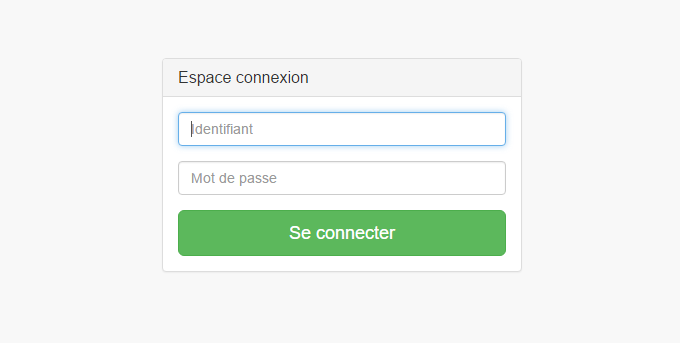
\includegraphics[width=9cm,height=4cm]{resultats/connexion.png}
\end{center}
%légende de l'image
\caption{Page de connexion}
\end{figure}
Le menu principal pour l’interface consacré au super administrateur contient quatre rubriques qui sont :
\begin{itemize}
\item Validation : cette rubrique contient toutes les notifications de validation qu’un super administrateur peut recevoir pour les valider. (Figure 5.2)\\
\item Gestion liste des utilisateurs : cette interface contient trois bouton ; un pour l’ajout d’un nouveau utilisateur, un deuxième pour modifier un compte déjà existant et un dernier pour supprimer un utilisateur. Cette interface est illustrée par la figure 5.3.\\
\item Message : contient un outil de communication entre les différents types d’exploitant (Figure 5.4).\\
\item Exception : cette rubrique est conçue pour gérer les opérations d’exception en cas d’urgence ou en cas d’enquête.\\
\end{itemize}

\begin{figure}[!h]
\begin{center}
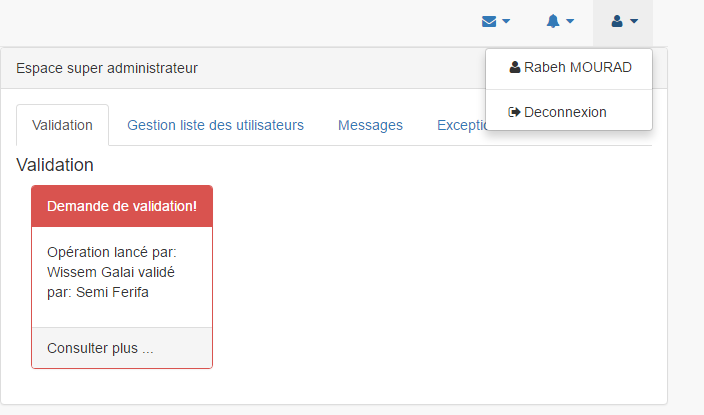
\includegraphics[width=10cm,height=4cm]{resultats/capture_validation.png}
\end{center}
%légende de l'image
\caption{Rubrique validation}
\end{figure}

\begin{figure}[!h]
\begin{center}
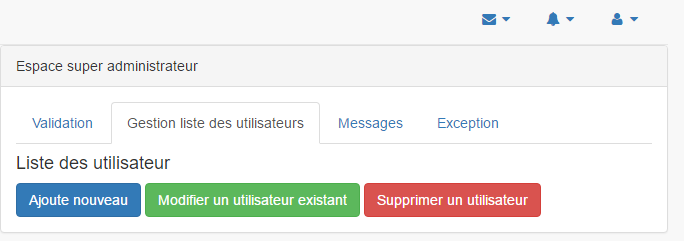
\includegraphics[width=10cm,height=6cm]{resultats/gestion.png}
\end{center}
%légende de l'image
\caption{Rubrique de gestion des utilisateurs}
\end{figure}

\begin{figure}[!h]
\begin{center}
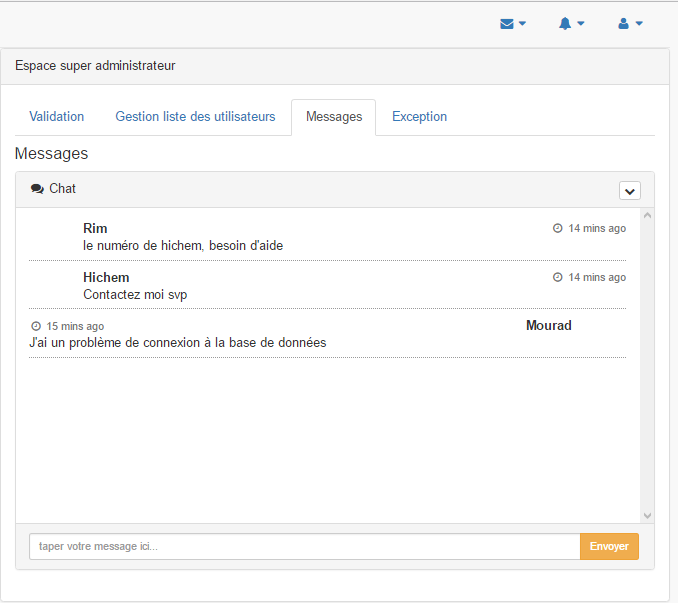
\includegraphics[width=10cm,height=6cm]{resultats/message.png}
\end{center}
%légende de l'image
\caption{Rubrique messages}
\end{figure}
\newpage
L’agent vérifie les NOTAM une à une pour les valider, cette validation se fait comme indiqué dans la figure 5.5. NB : le contenu de message dans la capture est un contenu à titre indicatif non pas le contenu réel des lignes de NOTAM.\\
\begin{figure}[!h]
\begin{center}
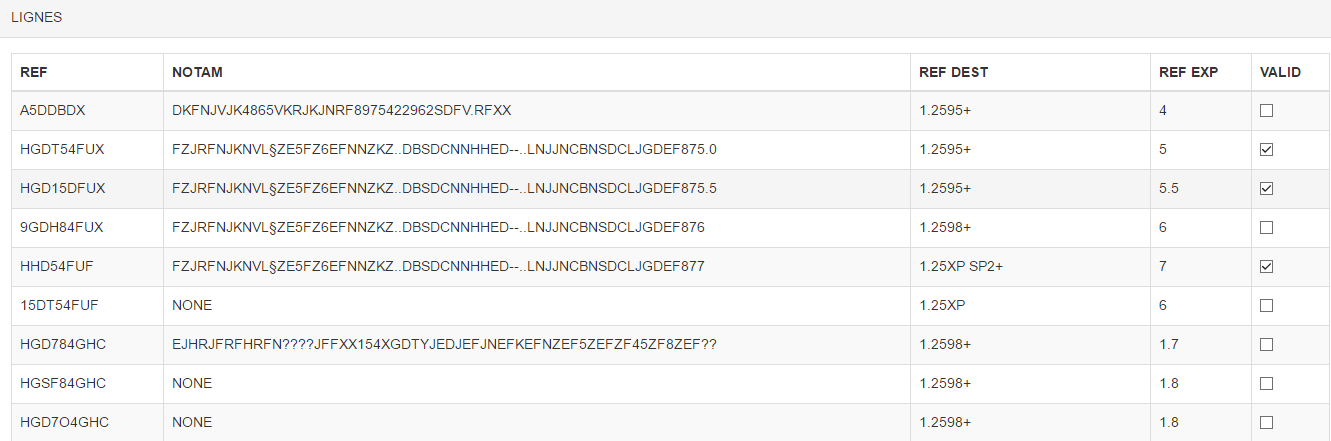
\includegraphics[width=15cm,height=6cm]{resultats/NOTAM.png}
\end{center}
%légende de l'image
\caption{Validation des lignes}
\end{figure}
\newpage
Après avoir validé les lignes à affecter, un agent configure la demande de validation puis la lance. Le traitement en cours de cette opération s’illustre par les figures 5.6, 5.7 et 5.8. \\
\begin{figure}[!h]
\begin{center}
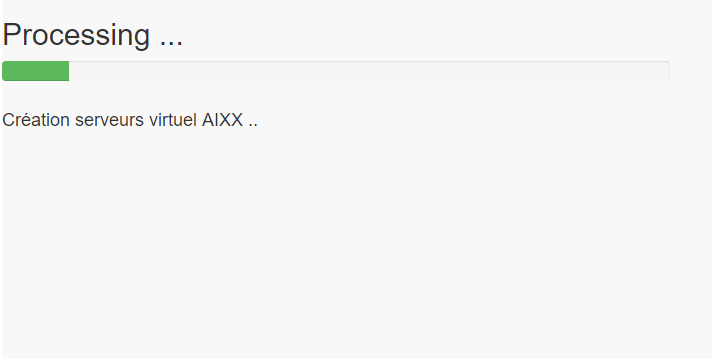
\includegraphics[width=10cm,height=6cm]{resultats/processing1.png}
\end{center}
%légende de l'image
\caption{Création du serveur virtuel AIXX}
\end{figure}

\begin{figure}[!h]
\begin{center}
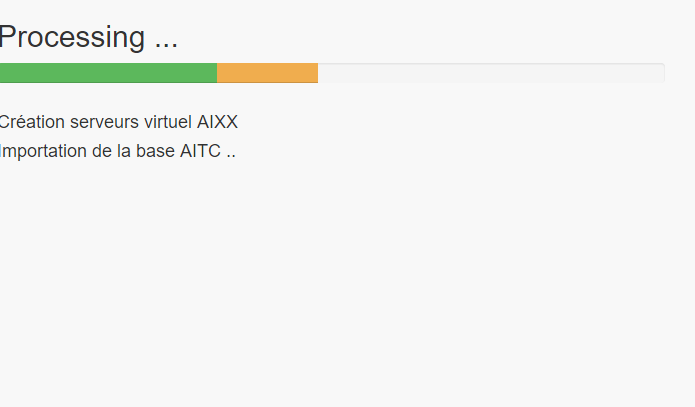
\includegraphics[width=10cm,height=6cm]{resultats/processing2.png}
\end{center}
%légende de l'image
\caption{Importation de la base AITC}
\end{figure}

\begin{figure}[!h]
\begin{center}
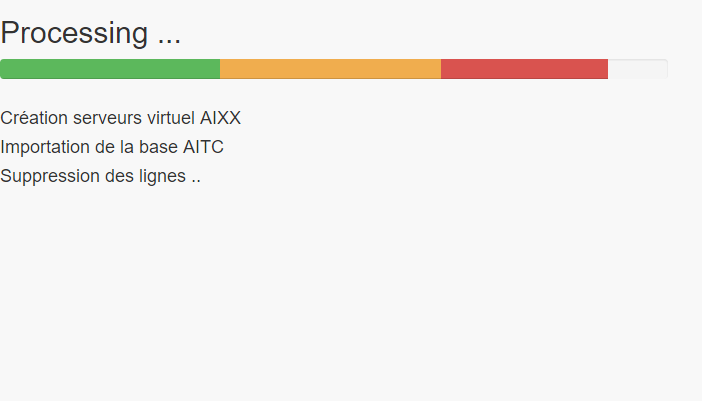
\includegraphics[width=10cm,height=6cm]{resultats/processing3.png}
\end{center}
%légende de l'image
\caption{Suppression des lignes NOTAM}
\end{figure}

\newpage


\section*{Conclusion}
Dans ce chapitre, nous avons présenté l’environnement et les technologies que nous avons
utilisées pour développer notre application. La première section de ce chapitre est réservée
à la présentation de l’environnement de travail utilisé. La deuxième section a été consacrée
à l’étude des choix techniques. La troisième section a exposé les principales interfaces réalisées
pour donner un aperçu sur le fonctionnement de l’application et le passage entre ses différentes
fenêtres.
